%%%%%%%%%%%%%%%%%%%%%%%%%%%%%%%%%%%%%%%%%
% Beamer Presentation
% LaTeX Template
% Version 1.0 (10/11/12)
%
% This template has been downloaded from:
% http://www.LaTeXTemplates.com
%
% License:
% CC BY-NC-SA 3.0 (http://creativecommons.org/licenses/by-nc-sa/3.0/)
%
% Modified by Jeremie Gillet in November 2015 to make an OIST Skill Pill template
%
%%%%%%%%%%%%%%%%%%%%%%%%%%%%%%%%%%%%%%%%%

%----------------------------------------------------------------------------------------
%	PACKAGES AND THEMES
%----------------------------------------------------------------------------------------

\documentclass{beamer}

\mode<presentation> {

\usetheme{Madrid}

\definecolor{OISTcolor}{rgb}{0.65,0.16,0.16}
\usecolortheme[named=OISTcolor]{structure}

%\setbeamertemplate{footline} % To remove the footer line in all slides uncomment this line
%\setbeamertemplate{footline}[page number] % To replace the footer line in all slides with a simple slide count uncomment this line

\setbeamertemplate{navigation symbols}{} % To remove the navigation symbols from the bottom of all slides uncomment this line
}

\usepackage{graphicx} % Allows including images
\usepackage{booktabs} % Allows the use of \toprule, \midrule and \bottomrule in tables
\usepackage{textpos} % Use for positioning the Skill Pill logo
\usepackage{fancyvrb}
\usepackage{tikz}
\usepackage{hyperref}
\usepackage{listings}
\usepackage{subfig}
%\usepackage{enumitem}
%\usepackage{calc}

\definecolor{dkgreen}{rgb}{0,0.6,0}
\definecolor{gray}{rgb}{0.5,0.5,0.5}
\definecolor{mauve}{rgb}{0.58,0,0.82}

\lstset{frame=tb,
  language=python,
  aboveskip=3mm,
  belowskip=3mm,
  showstringspaces=false,
  columns=flexible,
  basicstyle={\small\ttfamily},
  numbers=none,
  numberstyle=\tiny\color{gray},
  keywordstyle=\color{blue},
  commentstyle=\color{dkgreen},
  stringstyle=\color{mauve},
  breaklines=true,
  breakatwhitespace=true,
  tabsize=3
}

\newcommand*{\lstitem}[1]{
  \setbox0\hbox{\lstinline{#1}}  
  \item[\usebox0]  
  % \item[\hbox{\lstinline{#1}}]
  \hfill \\
}

%----------------------------------------------------------------------------------------
%	TITLE PAGE
%----------------------------------------------------------------------------------------

\title[Skill Pill]{Skill Pill: Julia} % The short title appears at the bottom of every slide, the full title is only on the title page
\subtitle{Lecture 2: Data Processing and Plotting}

\author{Ankur Dhar \& James Schloss} % Your name
\institute[OIST] % Your institution as it will appear on the bottom of every slide, may be shorthand to save space
{
	\textit{ankurd@oist.jp} \\ % Your institution for the title page
	\textit{james.schloss@oist.jp} % Your email address
}
\date{July 12, 2019} % Date, can be changed to a custom date

\begin{document}

\setbeamertemplate{background}{
\includegraphics[width=\paperwidth]{SPbackground.png}} % Adding the background logo

\begin{frame}
\vspace*{1.4cm}
\titlepage % Print the title page as the first slide
\end{frame}

\setbeamertemplate{background}{} % No background logo after title frame

\addtobeamertemplate{frametitle}{}{% Adding the Skill Pill logo on the title screen after title frame
\begin{textblock*}{100mm}(.92\textwidth,-0.9cm)

\includegraphics[height=0.85cm]{julia.pdf}
\end{textblock*}}

\begin{frame}
  \tableofcontents
\end{frame}
\section{Arrays}
\begin{frame}[fragile]{Creating Arrays}
	Arrays in Julia are defined very similarly to arrays in Matlab, using square brackets to denote them. By default arrays are row vectors, but can be transposed to column vectors.
	\begin{lstlisting}
	julia> x = [1 2 3 4]
	julia> y = collect(1:4)
	julia> z=[1;2;3;4]
	julia> w=x'
	julia> array = Int64[]
	\end{lstlisting}
	In addition sequences of numbers can be generated using the \verb|:| operator (start:step:end). To see all these values expanded out you will need to print them manually or use the \verb|collect| function. 
\end{frame}

\begin{frame}[fragile]{Array Generation Functions}
	\begin{description}[leftmargin=*]
		\item[zeros(S)] Makes an array of size S filled with zeros  
		\item[ones(S)]  Makes an array of size S filled with ones 
		\item[repeat(A,c,r)] Repeats array A column-wise c times and row-wise r times
		\item[rand(S)] Generates array of size S with random numbers between 0 and 1
		\item[Type\textbf{[]}] Creates empty array of type Type
	\end{description}
	
\end{frame}

\begin{frame}[fragile]{Array Operations}
	Arrays can be indexed by using square brackets after the array. For multidimensional arrays, the first dimension is the row, followed by column and so on. Output of indexing arrays is by default a column. This is crucial when it comes to multiplying arrays by each other.
	\begin{lstlisting}
	julia> data=rand(50,50)
	julia> rowdata=data[1,:]
	julia> inner = x*y
	julia> outer = y*x
	julia> square = x.*x
	\end{lstlisting}
	To execute scaler operations on an array, you can use append a \verb|.| to the operator. This is also applicate to functions which acts on scalars as well.
\end{frame}

\section{Data Handling}

\begin{frame}[fragile]{File Structure}
	To begin working with files, you must know where your working directory is. When launching Julia from an application menu (Windows/MacOS), the default directory is predefined. For Linux it will be the home directory. 
	\begin{lstlisting}
	julia> pwd()
	julia> cd("C:\\Users\\M\\Documents\\JuliaStuff")
	julia> readdir()
		\end{lstlisting}
	You can use \verb|pwd()| to print your working directory, and \verb|cd()| to change it to whichever new directory you would like.	Once you are in the directory you want, you can list the files within using \verb|readdir()|.
\end{frame}

\begin{frame}[fragile]{Writing Scripts}
	As we start to get into more complex commands and chain them together, we can use scripts to automatically execute a series of commands at once. To include these commands into the REPL, we simply use the \verb|include()| command 
	\begin{lstlisting}
	julia> include("Lesson 2.jl")
	julia> randflips[1];
	\end{lstlisting}
	To help debug in these scripts, you can suppress the direct output from any commands with a \verb|;|, and forcibly print values using \verb|print()| or \verb|println|.
\end{frame}

\begin{frame}[fragile]{Delimited text}
	The simplest data files are often delimited text files or CSV files, which can be manipulated like any other variable in Julia. To load any general delimited file, load the DelimitedFiles package. Reading in these files will automatically generate 1D or 2D arrays depending on the data being read in.
	\begin{lstlisting}
	julia> using DelimitedFiles
	julia> randData=readdlm("Random.txt")
	julia> writedlm(randData,"Random.csv")
	\end{lstlisting}
	Similarly, any 1D or 2D can be written to a file, with the actual delimiter being based on the file extension used (txt for space and csv for comma).
\end{frame}

\begin{frame}[fragile]{CSV files}
	Typical CSV files are a bit more complex than standard delimited files, with headers or labels. For this use case the CSV package is recommended. When reading in a file, the first row will be taken as the header row, but this can be explicitly defined.
	\begin{lstlisting}
	julia> using CSV
	julia> data = CSV.read("simplemaps-worldcities-basic.csv")
	julia> names(data)
	julia> populations = data[:pop]
	\end{lstlisting}
	Once read in, the labels along the header row can also be used to reference each column of data, so numeric indexing is not not necessary.
\end{frame}

\begin{frame}[fragile]{Exercises}
	\begin{block}{Exercise 1}
		Creates a file \verb|squares.txt| consisting of the first 5 square numbers
	\end{block}
	\begin{block}{Exercise 2}
		Write a script which creates a new file called \verb|large_cities.txt|.
		The file should contain one line for each of the cities which have a
		population larger than 10,000,000., formatted as follows:\\
		Buenos Aires, Argentina: population 11862073\\
		Sao Paulo, Brazil: population 14433147.5\\
		...
	\end{block}
\end{frame}

\section{Plotting}
\begin{frame}[fragile]{Plots in a Nutshell}
	\begin{columns}
		\column{.6\linewidth}
			To start with, let's add and load the general Plots package
		\begin{lstlisting}
		(v1.1) pkg> add Plots
		julia> using Plots
		julia> plot(Plots.fakedata(50))
		\end{lstlisting}
		This will let us call the general Plot commands, in this case \verb|plot| plots 1D data as a line plot.
		
		More information can be found at \url{https://docs.juliaplots.org/latest/}
		\column{.4\linewidth}
		\begin{figure}
			\centering
			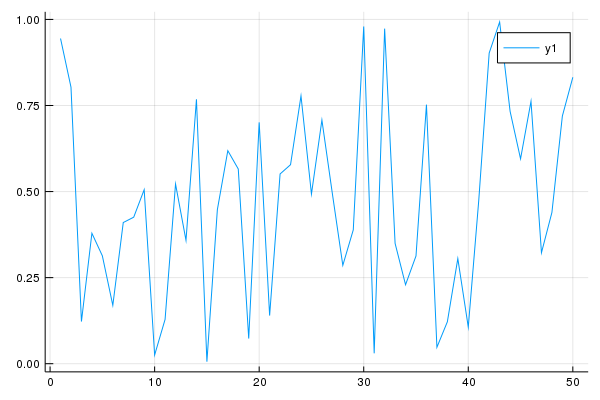
\includegraphics[width=\textwidth]{randPlot}
		\end{figure}
	\end{columns}
\end{frame}


\begin{frame}[fragile]{Plotting Commands}
	\begin{description}[leftmargin=*,align=right]
		\item[scatter(X,Y)] Scatter plot data with XY coordinates
		\item[bar(x,y)] Bar plot following similar rules to plot
		\item[histogram(x,bins=n)] Plots histogram of 1D data in n bins.
		\item[plot($\theta$,r,proj=:polar)] Polar plot of data following r and $\theta$
		\item[heatmap(x,y,z)] Plots heatmap following XY axes with intensity array z
		\item[fakedata(L,S)] Generates random S numbers of series data of length L
		\item[savefig(filename)] Saves a generated plot as an image file
	\end{description}
	
\end{frame}

\begin{frame}[fragile]{Plotting 3D Data}
%%TODO include heatmap, surf, and contour
	\begin{columns}
		\column{.6\textwidth}
		There are a couple of additional options for plotting 3D data:
		\begin{description}[align=right]
			\item[surface(x,y,z)] Draws surface in 3D space
			\item[contour(x,y,z)] Draws contours on 2D plane
		\end{description}
		The plotting commands \verb|plot|,\verb|scatter|,\verb|bar|, and \verb|heatmap| also can accept 3D data.
		\column{.4\textwidth}
		\begin{figure}
			\centering
			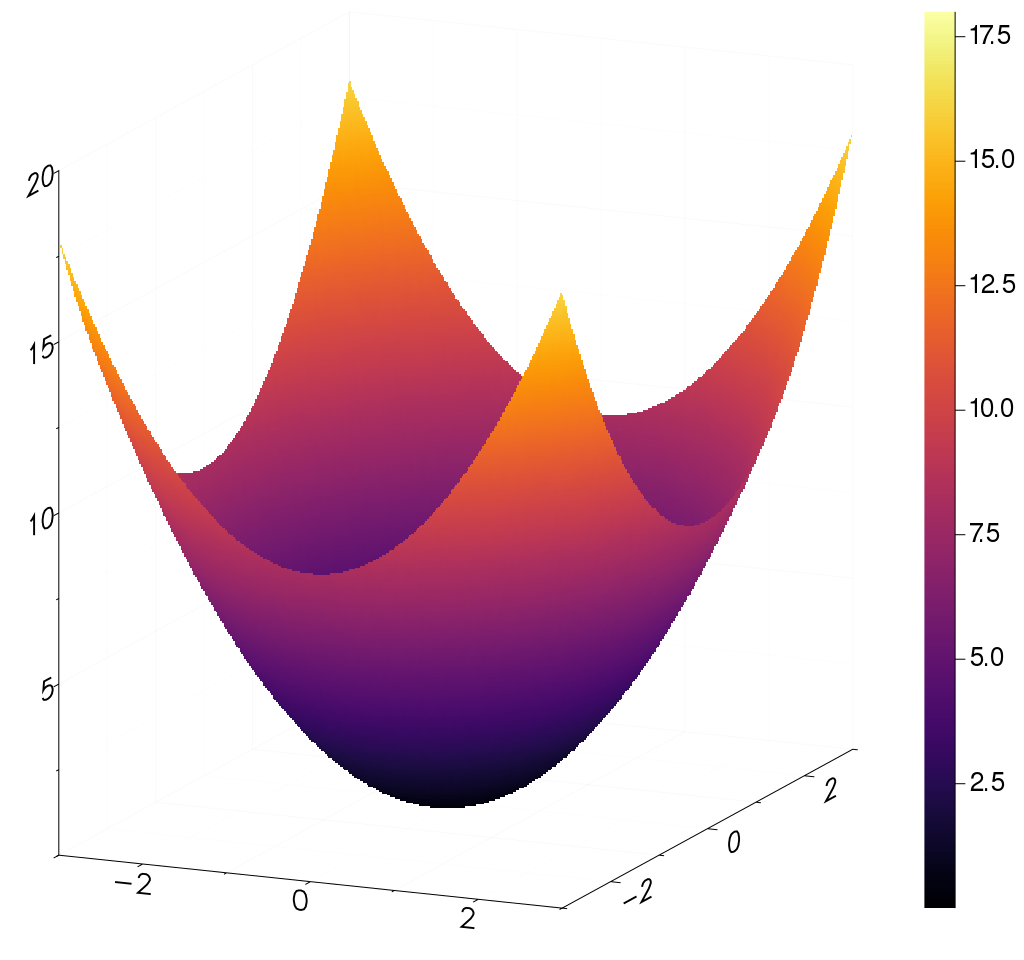
\includegraphics[width=\textwidth]{surf}
		\end{figure}
	\end{columns}
\end{frame}

\begin{frame}[fragile]{Plotting Vector Data}
	\begin{columns}
	\column{.5\textwidth}
	For vector data the current option is quiver:
	\begin{lstlisting}
	help?> quiver
	search: quiver quiver!
	
	quiver(x,y,quiver=(u,v))
	quiver!(x,y,quiver=(u,v))
	
	Make a quiver (vector field) plot. The ith vector extends from (x[i],y[i]) to (x[i] + u[i], y[i] + v[i]).
	\end{lstlisting}
	\column{.5\textwidth}
	\begin{figure}
		\centering
		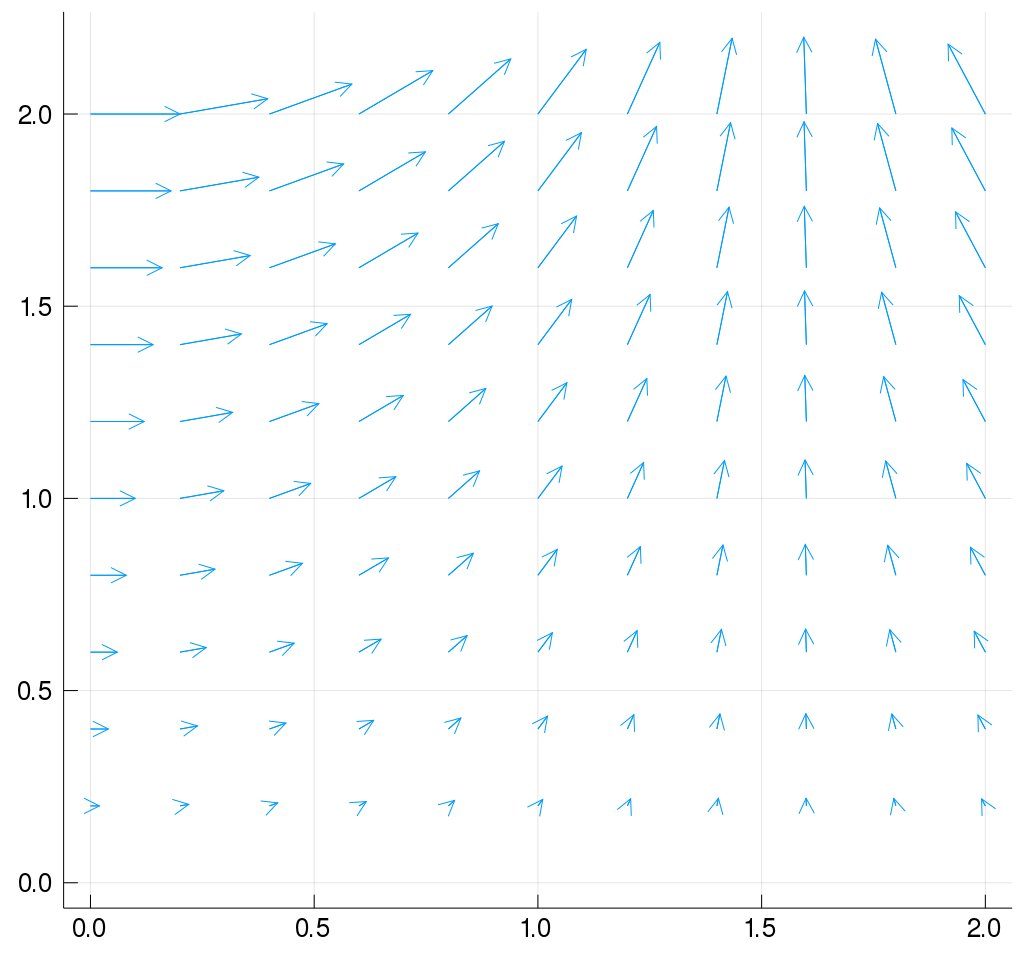
\includegraphics[width=\textwidth]{quiver}
	\end{figure}
\end{columns}

\end{frame}

\begin{frame}[fragile]{Plotting Backends}
	\begin{columns}
	\column{.5\linewidth}
	These commands are agnostic to the plotting backend, meaning they will work with a number of plotting engines in similar fashion. Each backend has pros and cons, but most commonly used are GR and PyPlot.
	
	\begin{figure}[h]
		\centering
		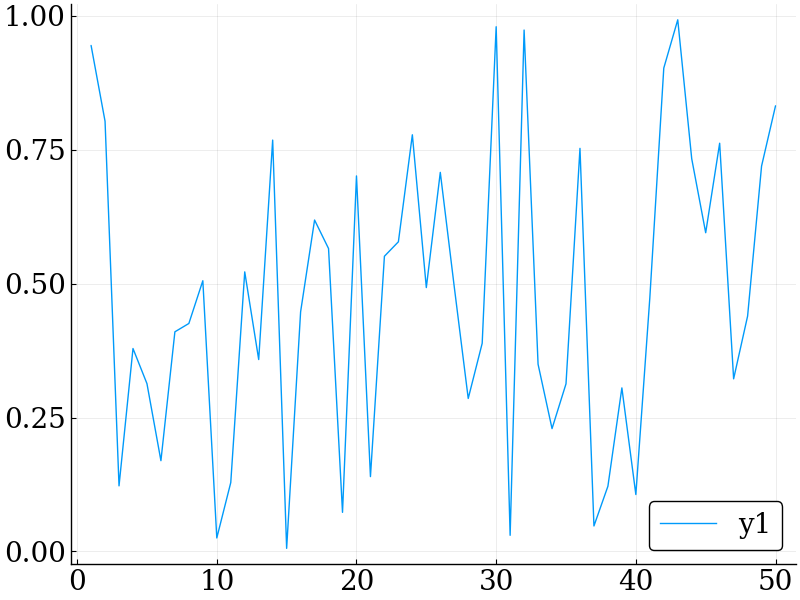
\includegraphics[width=.8\textwidth]{randPlotPy}
		\caption{PyPlot}
	\end{figure}

	\column{.5\linewidth}
	\begin{figure}[h]
		\centering
		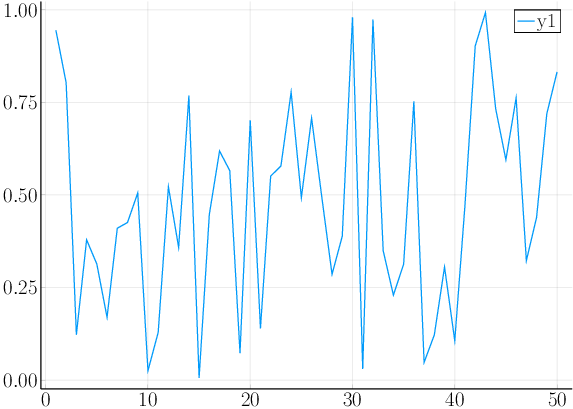
\includegraphics[width=.8\textwidth]{randPlotPGF}
		\caption{PGFPlots}
	\end{figure}
	\vspace{-11mm}
	\begin{figure}[h]
		\centering
		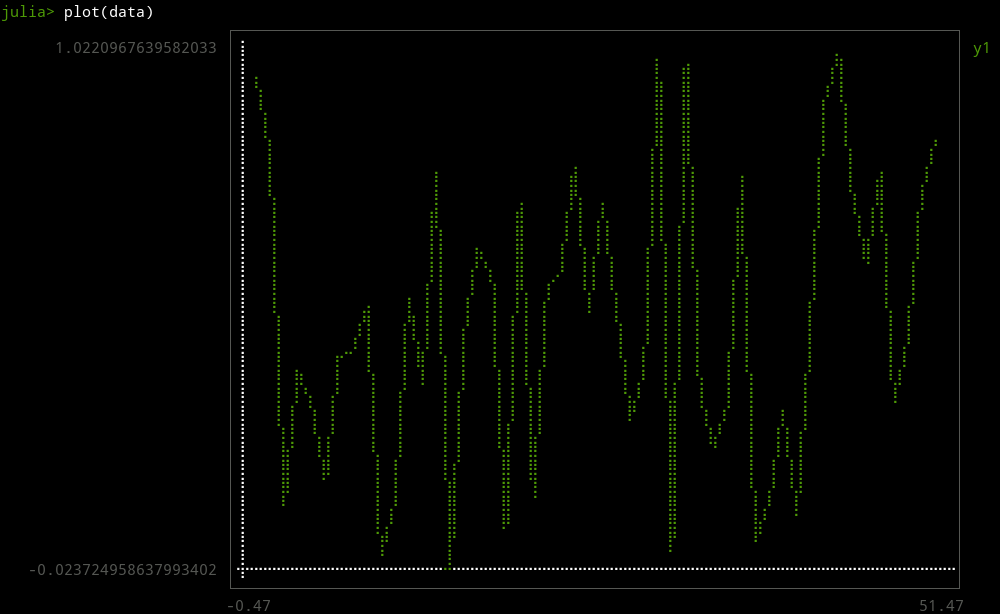
\includegraphics[width=.8\textwidth]{randPlotUni}
		\caption{UnicodePlots}
	\end{figure}
	\end{columns}
\end{frame}

\begin{frame}[fragile]{Formatting Commands}
Each of these commands can be expressed in-line with the plotting command or beforehand within a call to the plotting backend.
\begin{description}[leftmargin=*,align=right]
	\item[font(fontname,size)] Defines a Font object with a given size
	\item[size=(X,Y)] Sets size of plot to X by Y pixels
	\item[xlabel=string] Sets X-Y labels to string, also ylabel
	\item[title=string] Sets title to string, also colorbar\_title for heatmap.
	\item[xtickfont=font] Sets the font of x tick marks, also ytickfont,titlefont,guidefont
	\item[left\_margin=length] Sets margin for left side of plot, also top\_margin, bottom\_margin, and right\_margin
	\item[xscale=:log10] Sets x scale to log10, also yscale
\end{description}

\end{frame}


\begin{frame}[fragile]{Exercises}
	\begin{block}{Exercise 3}
		Read data.txt given in the Public Folder and plot the results.
		What do you see?
	\end{block}
	\begin{block}{Exercise 4}
		Plot a histogram of the longitudes of the world's cities. What is the mean and median longitude?
\end{block}

\end{frame}


\begin{frame}{What is next?}
  \begin{description}
    \item[Last Session] Problem Sets with James
    \item[Also next week] Advanced Topics with Valentin!
  \end{description}
\end{frame}
%\begin{frame}[fragile]{Using Fortran and C in Julia}
%	
%	Julia allows you to use other languages (such as Fortran or C) by using the \texttt{ccall} function:
%	
%	\begin{lstlisting}
%	julia> t = ccall((:clock, "libc"), Int32, ())
%	2292761
%	\end{lstlisting}
%	
%	Here, we are calling the \texttt{clock} function from the \texttt{libc} library in C.
%	
%\end{frame}
\end{document}
